\documentclass{article}
\usepackage[utf8]{inputenc}
\usepackage{amsmath, amssymb}
\usepackage{pgfplots}
\usepackage{breqn} % For automatic line breaking of long equations
\pgfplotsset{compat=1.18}
\usepackage{geometry}
 \geometry{a4paper, margin=1in}

\begin{document}

\begin{center}
\section*{SVT by an even 4 degree polynomial}
\end{center}

%===========================================================================
%
%. What does SVT do?
%
%===========================================================================

\subsection*{What does SVT do?}
In this note, we will show how to perform a polynomial transformation of the singular values of some matrix $A$.
We will do so in a specific example with the polynomial 
$$
p(x) = \frac{1}{2}x^4 + \frac{1}{2}x^2
$$
As the result of the transformation, the singular values values $\sigma_i$ well be transformed into
$$
\sigma_i \rightarrow p(\sigma_i)
$$
It is required that $A$ is embedded in the upper left corner of a unitary matrix $U_A$. 
$$
	\Pi U_A \Pi = \begin{pmatrix} A & 0 \\ 0 & 0 \end{pmatrix}
$$
for a suitable projection matrix $\Pi$. This unitary embedding/encoding is what makes SVT suitable for quantum computation. Notice that no prior knowledge of the singular values (or vectors) are required for the SVT to work.



%===========================================================================
%
%. Conditions for SVT and why it works
%
%===========================================================================

\subsection*{Conditions for SVT and why it works}

\noindent The process of SVT can roughly be divided into two steps: \\ 

\noindent The first step is Quantum Signal Processing (QSP) where $2\times 2$ matrices of the form
$$
W(x) = \begin{bmatrix}
x & i\sqrt{1-x^2} \\
i\sqrt{1-x^2} & x
\end{bmatrix}
$$
gets transformed according to the following theorem by Gilyen et al.\\

\noindent  \textbf{Theorem 1 (QSP)} \\
\textit{There exist} $\Psi_{P,Q} = \{\phi_0, \phi_1, \dots, \phi_k\} \in \mathbb{R}^{k+1}$ \textit{ such that for all } $x \in [-1, 1]:$
$$
e^{i\phi_0 \sigma_z} \prod_{j=1}^{k} (W(x)e^{i\phi_j \sigma_z}) = 
\begin{bmatrix}
P(x) & iQ(x)\sqrt{1-x^2} \\
iQ^*(x)\sqrt{1-x^2} & P^*(x)
\end{bmatrix}
$$
\noindent \textit{if and only if  there exists a pair} $P, Q \in \mathbb{C}[x]$ \textit{ such that}
\begin{itemize}
    \item $\deg(P) \leq k \text{ and } \deg(Q) \leq k - 1$
    \item $P \text{ has parity-}(k \pmod 2) \text{ and } Q \text{ has parity-}(k - 1 \pmod 2)$
    \item $\forall x \in [-1, 1]:$ 
\begin{equation}    
    |P(x)|^2 + (1 - x^2)|Q(x)|^2 = 1 \label{eq:qsp_condition}
\end{equation}
\end{itemize}

\noindent Secondly the  SVT method (singular value transformation) uses the fact that $U_A$ can be broken down into scalar diagonal entries or $2\times 2$-blocks similar to $W(x)$'s, evaluated in the singular values, with respect to certain bases of left and right singular vectors and their orthogonal completions. So SVT is actually just QSP on these block parts. The relevant theorem is:\\

\noindent  \textbf{Theorem 2 (SVT)} \\
Let $\mathcal{H}$ be a finite-dimensional Hilbert space and let $U_A, \Pi, \tilde{\Pi} \in \text{End}(\mathcal{H})$ be linear operators on $\mathcal{H}$ such that $U_A$ is a unitary encoding of $A$, and $\Pi, \tilde{\Pi}$ are orthogonal projectors \footnote{In our case, where we look at a quadratic matrix $A$, we only need $\Pi$.}. 
Let $P \in \mathbb{C}[x]$ be a degree-$d$ polynomial satisfying
\begin{itemize}
    \item $P$ has parity-$(d \pmod 2)$,
    \item $\forall x \in [-1, 1]: |P(x)| \leq 1$,
    \item $\forall x \in (-\infty, -1] \cup [1, \infty): |P(x)| \geq 1$,
    \item if $d$ is even, then $\forall x \in \mathbb{R}: P(ix)P^*(ix) \geq 1$.
\end{itemize} 
then there exists a vector $\Phi_P \in \mathbb{R}^d$ such that the projected unitary
\begin{equation*}
P^{(SV)}(\tilde{\Pi}U\Pi) \equiv \begin{cases} \tilde{\Pi}U_\Phi\Pi & \text{if } n \text{ is odd, and} \\ \Pi U_\Phi\Pi & \text{if } n \text{ is even.} \end{cases}
\end{equation*}
has singular values $P(\sigma_i)$ where the $\sigma$'s are the singular values of $A$.\\

\noindent The matrix $U_\Phi$, called the alternating phase modulated sequence, is defined as 
$$
U_{\Phi} = \begin{cases} e^{i\phi_1(2\tilde{\Pi}-I)}U_A \prod_{j=1}^{(n-1)/2} \left( e^{i\phi_{2j}(2\Pi-I)}U_A^\dagger e^{i\phi_{2j+1}(2\tilde{\Pi}-I)}U_A \right) & \text{if } n \text{ is odd, and} \\ \prod_{j=1}^{n/2} \left( e^{i\phi_{2j-1}(2\Pi-I)}U_A^\dagger e^{i\phi_{2j}(2\tilde{\Pi}-I)}U_A \right) & \text{if } n \text{ is even.} \end{cases}
$$
This is the matrix we aim to calculate. In the following we will describe an algorithm to do exactly this.

%===========================================================================
%
% The algorithm
%
%===========================================================================

\subsection*{The algorithm}
As mentioned above, the point of this note, is not to prove that the assertions of the theorems are true. Instead we will describe an algorithm to calculate $U_{\Phi}$:

\begin{itemize}
    \item Starting with $p(x)$ we will find a pair of real polynomials $a(x)$ and $b(x)$ so that the complex polynomials
\begin{align*}
 P(x) & = p(x) + i \cdot a(x) \\
 Q(x) & = i \cdot b(x)
 \end{align*}
 satisfies the condition (\ref{eq:qsp_condition}).
    \item We can then use $P,Q$ to algorithmically construct the QSP vector $\Psi_{P,Q}$.
    \item The polynomial $P(x)$ actually also satisfies the conditions in Theorem 2, so we can transform the $\Psi_{P,Q}$ vector into a $\Phi_P$ vector
    \item Finally we calculate the $U_{\Phi}$
\end{itemize}

\noindent For the algorithm to work, we have chosen $p(x)$ so that it is an even real polynomial of degree four, satisfying the conditions
\begin{itemize}
    \item $p(x)$ has parity-($n \pmod 2$) and
    \item for all $x \in [-1, 1]: |p(x)| \leq 1$.
\end{itemize}

\noindent The second condition can easily be verified by graphing:
\begin{center}
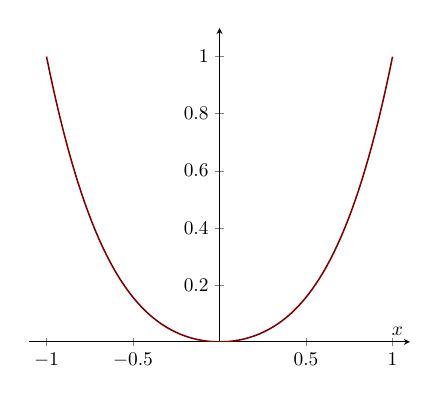
\begin{tikzpicture}[scale=0.7, transform shape]
\begin{axis}[
    axis lines = middle,
    xlabel = $x$,
    ymin=0, ymax=1.1,
    xmin=-1.1, xmax=1.1,
    ytick={0.2, 0.4, 0.6, 0.8, 1},
    xtick={-1, -0.5, 0, 0.5, 1},
    width=0.7\textwidth,
    height=0.6\textwidth,
]
\addplot [domain=-1:1, samples=100, color=red!50!black, thick] {0.5*x^4 + 0.5*x^2};
\end{axis}
\end{tikzpicture}
\end{center}

%===========================================================================
%
% Finding real polynomial pairs for QSP
%
%===========================================================================

\subsection*{Finding real polynomial pairs for QSP}

\noindent We want to find a pair of real polynomials $a(x)$ and $b(x)$ satisfying condition (\ref{eq:qsp_condition}).\\ 
In terms of the real polynomials we want to find, this is
\begin{equation*}
1 = |p(x) + i \cdot a(x)|^2 + (1-x^2) \cdot |b(x)|^2 
\end{equation*}

\noindent To do it, we start by finding the roots in the 1. quadrant of $\tilde{p}(x)$ defined as
\begin{equation}
1 - p(x)^2 = -\frac{1}{4}x^8 - \frac{1}{2}x^6 - \frac{1}{4}x^4 + 1 \equiv \tilde{p} (x) \label{eq:one_condition}
\end{equation}

\noindent  The relevant roots are
\[ x=1, x=i\sqrt{2}, x= \frac{\sqrt{2\sqrt{2}-1}}{2} + \frac{i\sqrt{2\sqrt{2}+1}}{2} \]

\noindent Plotting, we see that the polynomial is non-negative for all values in $[-1, 1]$ and so we can use the following procedure.
\begin{center}
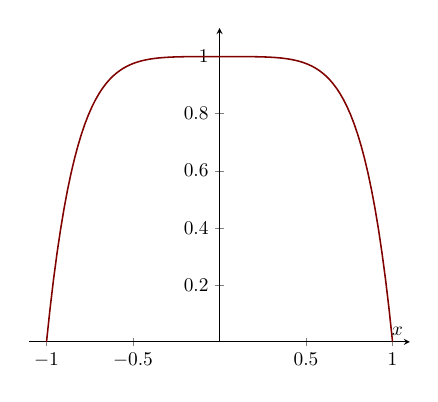
\begin{tikzpicture}[scale=0.7, transform shape]
\begin{axis}[
    axis lines = middle,
    xlabel = $x$,
    ymin=0, ymax=1.1,
    xmin=-1.1, xmax=1.1,
    ytick={0.2, 0.4, 0.6, 0.8, 1},
    xtick={-1, -0.5, 0, 0.5, 1},
    width=0.7\textwidth,
    height=0.6\textwidth,
]
\addplot [domain=-1:1, samples=100, color=red!50!black, thick] {1 - 0.25*x^8 - 0.5*x^6 - 0.25*x^4};
\end{axis}
\end{tikzpicture}
\end{center}

\noindent Let $\gamma_1 = 1$, $\gamma_2 = \sqrt{2}$ and $\gamma_3 = a+ib$ where
$$
a := \frac{\sqrt{2\sqrt{2}-1}}{2}, b := \frac{\sqrt{2\sqrt{2}+1}}{2}
$$

\noindent Letting 
$$
c := a^2 + b^2 + \sqrt{2 \cdot (a^2+1) \cdot b^2 + (a^2-1)^2 + b^4}
$$
we define:
\begin{align*}
    R(x) &:= \sqrt{(\gamma_1)^2 - 1} \cdot x + i \cdot \gamma_1 \cdot \sqrt{1-x^2} \\
    S(x) &:= \sqrt{(\gamma_2)^2 + 1} \cdot x + i \cdot \gamma_2 \cdot \sqrt{1-x^2} \\
    T(x) &:= (c \cdot x^2 - (a^2 + b^2)) + i \cdot \sqrt{c^2 - 1} \cdot x \cdot \sqrt{1-x^2}
\end{align*}

\noindent All of these three expressions have the same common form
$$
A(x) + i \cdot \sqrt{1-x^2} \cdot B(x)
$$
for some polynomials $A$ and $B$, and actually when multiplying such expressions they keep that form.\\

\noindent Furthermore the product $V(x) = 1/2\cdot R(x) \cdot S(x) \cdot T(x)$ has the property that
$$
\tilde{p}(x) = V(x) \cdot \overline{V(x)}
$$

\noindent Therefore it is not difficult to show by direct calculation, using definition (\ref{eq:one_condition}) for $\tilde{p}(x)$, that with 
$$
V(x) = a(x) + i \cdot \sqrt{1-x^2} \cdot b(x)
$$
the polynomials
\begin{align*}
P(x) & = p(x) + i \cdot a(x) \\
Q(x) & = i \cdot b(x)
\end{align*}
satisfy condition  (\ref{eq:qsp_condition}).\\

\noindent All that remains is to expand the product $\frac{1}{2}\cdot R(x)\cdot S(x)\cdot T(x)$ and we get
\begin{align*}
    a(x) &:= 5.241339430x^4 - 6.241339430x^2 + 0.9999999995 \\
    b(x) &:= 5.265134285x^3 - 3.533083477x
\end{align*}

%===========================================================================
%
% The QSP vector $\Psi$
%
%===========================================================================

\section*{The QSP vector $\Psi_{P,Q}$}

\noindent Now that we have a complex polynomial pair, 
\begin{align*}
    P(x) & = \left( \frac{1}{2} + 5.241339430 i \right) x^4 + \left( \frac{1}{2} - 6.241339430 i \right) x^2 + i \\
    Q(x) & = 5.265134285 i x^3 - 3.533083477 i x
\end{align*}
satisfying condition (\ref{eq:qsp_condition}) (and with $Re(P(x)) = p(x)$), we are in a position to find the quantum signal processing vector $\Psi_{P,Q}$. \\

\noindent The last element $\psi_4$ of the vector is found first. The quotient of the leading terms $P_4$ resp. $Q_3$ is unimoduler, thanks to (\ref{eq:qsp_condition}), so we let
\begin{align*}
    e^{i\frac{\psi_4}{2}} & = \frac{P_4}{Q_3} = \frac{0.5 + 5.241339430 i}{5.265134285 i}
\end{align*}

\noindent Solving for $\psi_4$ we get
\begin{align*}
    \psi_4 &= -0.04755382847
\end{align*}

\noindent Next we define two new polynomials 
\begin{align*}
    P^{(2)}(x) &= e^{-i \cdot \psi_4} (x \cdot P(x) + \frac{P_4}{Q_3} \cdot (1 - x^2) \cdot Q(x)) \\
    Q^{(2)}(x) &= e^{-i \cdot \psi_4} (\frac{P_4}{Q_3} \cdot x \cdot Q(x) - P(x))
\end{align*}
\noindent Because of the way we multiply with the quotient of leading terms, they are always both of lesser degree and opposite parity. In this case we get
\begin{align*}
    P^{(2)}(x) &= (1.2143537675 + 2.5777558080 i) x^3 \\
    &- (0.21548423776 + 2.5302199008 i) x  \\
    Q^{(2)}(x) &= 0.04753590769 - 0.9988695293 i \\
    &+ (-0.9640708301 + 2.68142639756 i) x^2 
\end{align*}
We now recursively form the quotient of leading terms, calculate $\psi_3$ define two new polynomials in the same manner as before, until we finally get
\begin{align*}
    P^{(5)}(x) &= 0.04753590765 + 0.99886952976 i \\
    Q^{(5)}(x) &= 0
\end{align*}
Notice that the leading term of $P^{(5)}(x)$ is unimodular. We let $e^{i\psi_0} = P^{(5)}(x)$ and obtain
$$
\psi_0 = 1.52324249839
$$

\noindent We have found the full QSP vector:
\begin{align*}
    \Psi_{P,Q} &= [1.52324249839, -0.3926990817, 0.69029050678, -0.3926990819, -0.047553828465 ]
\end{align*}

%===========================================================================
%
% The conditions in Theorem 2
%
%===========================================================================


\section*{The conditions in Theorem 2}

\noindent We  have to make sure the last three conditions on $P(x)$ in Theorem 2 is met. We do so graphically.\\
\noindent Plotting $P(x)\cdot P^*(x)$ we get

\begin{center}
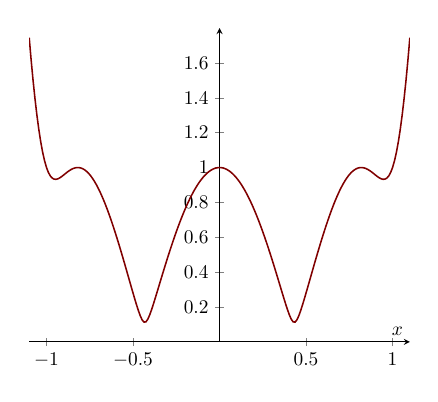
\begin{tikzpicture}[scale=0.7, transform shape]
\begin{axis}[
    axis lines = middle,
    xlabel = $x$,
    ymin=0, ymax=1.8,
    xmin=-1.1, xmax=1.1,
    ytick={0.2, 0.4, 0.6, 0.8, 1.0, 1.2, 1.4, 1.6},
    xtick={-1, -0.5, 0, 0.5, 1},
    width=0.7\textwidth,
    height=0.6\textwidth,
]
\addplot [domain=-1.1:1.1, samples=200, color=red!50!black, thick] 
{sqrt((0.5*x^4 + 0.5*x^2)^2 + (5.24133943*x^4 - 6.24133943*x^2 + 1)^2)};
\end{axis}
\end{tikzpicture}
\end{center}

\noindent This clearly matches
\begin{itemize}
    \item $\forall x \in [-1, 1]: |P(x)| \leq 1$,
    \item $\forall x \in (-\infty, -1] \cup [1, \infty): |P(x)| \geq 1$,
\end{itemize} 

\noindent Finally we plot $P(ix)\cdot P^*(ix)$
\begin{center}
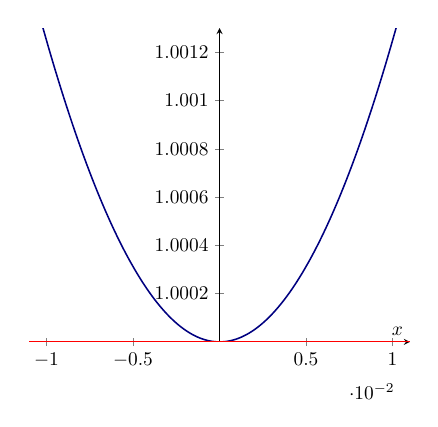
\begin{tikzpicture}[scale=0.7, transform shape]
\begin{axis}[
    axis lines = middle,
    xlabel = $x$,
    ymin=1, ymax=1.0013,
    xmin=-0.011, xmax=0.011,
    ytick={1.0002, 1.0004, 1.0006, 1.0008, 1.0010, 1.0012},
    xtick={-0.010, -0.005, 0, 0.005, 0.010},
    width=0.7\textwidth,
    height=0.6\textwidth,
    y tick label style={/pgf/number format/fixed, /pgf/number format/precision=4}
]
\addplot [domain=-0.011:0.011, samples=200, color=blue!50!black, thick] 
{27.721639*x^8 + 64.92595*x^6 + 49.68699*x^4 + 12.48267*x^2 + 1};
\addplot [domain=-0.011:0.011, color=red, thick] {1};
\end{axis}
\end{tikzpicture}
\end{center}
and we can visuallly confirm that the last condition
\begin{itemize}
    \item if $d$ is even, then $\forall x \in \mathbb{R}: P(ix)P^*(ix) \geq 1$.
\end{itemize} 
is also met.

%===========================================================================
%
% The SVT vector $\Phi$}
%
%===========================================================================


\section*{The SVT vector $\Phi_P$}

\noindent Given the QSP vector $\Psi_{P,Q}$ , we make the transformation to the SVT vector $\Phi_P$:
$$
 \phi_1 = \psi_0 + \psi_d + (d - 1)\frac{\pi}{2} 
 $$
 In our case $d=4$. And for all other $j \in \{2, \dots, d \}$
 $$
 \phi_j = \psi_{j-1} - \frac{\pi}{2}
$$
We get
\begin{align*}
    \Phi & = \left[ \psi_0 + \psi_4 + \frac{(4-1)\pi}{2}, \psi_1 - \frac{\pi}{2}, \psi_2 - \frac{\pi}{2}, \psi_3 - \frac{\pi}{2} \right] \\
           & = [ 6.1880776503, -1.9634954085, - 2.2610868336, -1.96349540869 ]
\end{align*}

\noindent The only reason why we do this final transformation is technical. In the paper by Gilyen et al., the matrix $W$ introduced earlier, is replaced by a single qubit reflection matrix
$$
\begin{bmatrix}
x & \sqrt{1 - x^2} \\
\sqrt{1 - x^2} & -x
\end{bmatrix}
$$
It is meant to "fit the block-encoding formalism nicer".\\

\noindent Finally we have all the ingredients we need to do a singular value tranformation for some unitarily encoded test matrix $A$.

%===========================================================================
%
% The SVT vector $\Phi$}
%
%===========================================================================

\section*{Testing an SVT}

\noindent To test SVT, we conveniently define a test matrix using an SVD:
$$
    U = \begin{bmatrix} \frac{\sqrt{3}}{2} & -\frac{1}{2} \\ \frac{1}{2} & \frac{\sqrt{3}}{2} \end{bmatrix} ,
    S = \begin{bmatrix}  \frac{8}{10}         & 0    \\   0 & \frac{6}{10} \end{bmatrix} ,
    V = \begin{bmatrix} \frac{1}{\sqrt{2}} & -\frac{1}{\sqrt{2}} \\ \frac{1}{\sqrt{2}} & \frac{1}{\sqrt{2}}\end{bmatrix} 
$$
The singular values are the diagonal entries in $S$, and the our matrix is the product 
\begin{align*}
    A & = U \cdot S \cdot V  \\
       & =  \begin{bmatrix} \frac{\sqrt{3} \sqrt{2}}{5} - \frac{3 \sqrt{2}}{20} & -\frac{\sqrt{3} \sqrt{2}}{5} - \frac{3 \sqrt{2}}{20} \\
\frac{\sqrt{2}}{5} + \frac{3 \sqrt{3} \sqrt{2}}{20} & -\frac{\sqrt{2}}{5} + \frac{3 \sqrt{3} \sqrt{2}}{20}
\end{bmatrix}
\end{align*}
The only reason we construct a matrix this way, is for test purposes. We repeat that the actual SVT does not require of us to know the singular values in advance. (But if we don't know them, it's hard to tell if the results are a match :-)\\

\noindent We encode $A$ in a Halmos dilation unitary  $U_A$:
\begin{align*}
    U_A & = \begin{pmatrix} A & (I - AA^{\dagger})^{1/2} \\ (I - A^{\dagger}A)^{1/2} & -A^{\dagger} \end{pmatrix}\\
& =
\begin{bmatrix}
\frac{\sqrt{3}\sqrt{2}}{5} - \frac{3\sqrt{2}}{20} & -\frac{\sqrt{3}\sqrt{2}}{5} - \frac{3\sqrt{2}}{20} & \frac{13}{20} & -\frac{\sqrt{3}}{20} \\
\frac{\sqrt{2}}{5} + \frac{3\sqrt{3}\sqrt{2}}{20} & -\frac{\sqrt{2}}{5} + \frac{3\sqrt{3}\sqrt{2}}{20} & -\frac{\sqrt{3}}{20} & \frac{3}{4} \\
\frac{7}{10} & \frac{1}{10} & -\frac{\sqrt{3}\sqrt{2}}{5} + \frac{3\sqrt{2}}{20} & -\frac{\sqrt{2}}{5} - \frac{3\sqrt{3}\sqrt{2}}{20} \\
\frac{1}{10} & \frac{7}{10} & \frac{\sqrt{3}\sqrt{2}}{5} + \frac{3\sqrt{2}}{20} & \frac{\sqrt{2}}{5} - \frac{3\sqrt{3}\sqrt{2}}{20}
\end{bmatrix}
\end{align*}

\noindent Obviously we have 
\begin{align*}
	\Pi U_A \Pi & = \begin{pmatrix} A & 0 \\ 0 & 0 \end{pmatrix}
\end{align*}

\noindent when we define the projection
\begin{align*}
    \Pi &= \begin{bmatrix} 1 & 0 & 0 & 0 \\ 0 & 1 & 0 & 0 \\ 0 & 0 & 0 & 0 \\ 0 & 0 & 0 & 0 \end{bmatrix} 
\end{align*}

\noindent We then calculate the alternating phase modulating sequence for $\Phi_P$:
\begin{align*}
 P(\Pi U_A \Pi) & =  \Pi \cdot e^{i\cdot\phi_1\cdot(2\Pi - I)} \cdot U_A^{\dagger} \cdot e^{i\cdot\phi_2\cdot(2\Pi - I)} \cdot U_A \cdot e^{i\cdot\phi_3\cdot(2\Pi - I)} \cdot U_A^{\dagger} \cdot e^{i\cdot\phi_4\cdot(2\Pi - I)} \cdot U_A \cdot \Pi \\
 & = \begin{bmatrix}
0.3848000001 - 0.7076046052i & -0.1400000000 + 0.1400000000i & 0. & 0. \\
-0.1400000000 + 0.1400000000i & 0.3848000001 - 0.7076046052i & 0. & 0. \\
0. & 0. & 0. & 0. \\
0. & 0. & 0. & 0.
\end{bmatrix}
\end{align*}

\noindent Observe that the "phase matrices" are diagonals
\begin{align*}
    e^{i \cdot \phi_i \cdot (2\Pi - I)} &= \begin{bmatrix} e^{i \cdot \phi_i} & 0 & 0 & 0 \\ 0 & e^{i \cdot \phi_i} & 0 & 0 \\ 0 & 0 & e^{-i \cdot \phi_i} & 0 \\ 0 & 0 & 0 & e^{-i \cdot \phi_i} \end{bmatrix} 
\end{align*}

\noindent  We now have a matrix which is transformed by $P(x)$. But to get the resulting matrix, with singular values $p(\sigma_i)$, we also need the SVT using the complex conjugate polynomial $P^*(x)$:
\begin{align*}
 P^*(\Pi U_A \Pi) & =  \Pi \cdot e^{-i\cdot\phi_1\cdot(2\Pi - I)} \cdot U_A^{\dagger} \cdot e^{-i\cdot\phi_2\cdot(2\Pi - I)} \cdot U_A \cdot e^{-i\cdot\phi_3\cdot(2\Pi - I)} \cdot U_A^{\dagger} \cdot e^{-i\cdot\phi_4\cdot(2\Pi - I)} \cdot U_A \cdot \Pi\\
& = \begin{bmatrix}
0.3848000001 + 0.7076046052i & -0.1400000000 - 0.1400000000i & 0. & 0. \\
-0.1400000000 - 0.1400000000i & 0.3848000001 + 0.7076046052i & 0. & 0. \\
0. & 0. & 0. & 0. \\
0. & 0. & 0. & 0.
\end{bmatrix}
\end{align*}

\noindent The final result is the average of these two contributions. The result of finding the singular values are:
\begin{align*}
    &SV \left( \frac{P(\Pi U_A \Pi)}{2} + \frac{P^*(\Pi U_A \Pi)}{2} \right) \\
    &= \begin{bmatrix} 0.52480000005 \\ 0.24480000005 \\ 0. \\ 0. \end{bmatrix} 
\end{align*}

\noindent It is seen to match the desired results with high accuracy:
\begin{align*}
    p(0.8) &= 0.52480  \\
    p(0.6) &= 0.24480
\end{align*}

\end{document}
